\documentclass[16pt]{beamer}

\ifdefined\chinchin
\usepackage[CJKspace]{xeCJK}
%\setCJKmainfont[BoldFont=SimHei,ItalicFont=AR PL KaitiM GB]{Alibaba PuHuiTi}
\setCJKmainfont{Alibaba PuHuiTi}
\newcommand{\cc}[2]{#1}
\else
\newcommand{\cc}[2]{#2}
\fi

%\usepackage{newtxtext,newtxmath}	% use Times Roman font
%\usepackage{newtxtext}
%\renewcommand{\familydefault}{\sfdefault}
%\usefonttheme{serif}
\usefonttheme{professionalfonts}
%\setbeamertemplate{theorems}[numbered]
\setbeamertemplate{caption}{\insertcaption} 	% no `Figure' prefix before caption

\mode<presentation> {

%\usetheme{default}
%\usetheme{AnnArbor}
%\usetheme{Antibes}
%\usetheme{Bergen}
%\usetheme{Berkeley}
%\usetheme{Berlin}
%\usetheme{Boadilla}
%\usetheme{CambridgeUS}
%\usetheme{Copenhagen}
%\usetheme{Darmstadt}
%\usetheme{Dresden}
%\usetheme{Frankfurt}
%\usetheme{Goettingen}
%\usetheme{Hannover}
%\usetheme{Ilmenau}
%\usetheme{JuanLesPins}
%\usetheme{Luebeck}
\usetheme{Madrid}
%\usetheme{Malmoe}
%\usetheme{Marburg}
%\usetheme{Montpellier}
%\usetheme{PaloAlto}
%\usetheme{Pittsburgh}
%\usetheme{Rochester}
%\usetheme{Singapore}
%\usetheme{Szeged}
%\usetheme{Warsaw}

%\usecolortheme{albatross}
%\usecolortheme{beaver}
%\usecolortheme{beetle}
%\usecolortheme{crane}
%\usecolortheme{dolphin}
%\usecolortheme{dove}
%\usecolortheme{fly}
%\usecolortheme{lily}
\usecolortheme{orchid}
%\usecolortheme{rose}
%\usecolortheme{seagull}
%\usecolortheme{seahorse}
%\usecolortheme{whale}
%\usecolortheme{wolverine}		% Hofstra

%\setbeamertemplate{footline} % To remove the footer line in all slides uncomment this line
\setbeamertemplate{footline}[page number] % To replace the footer line in all slides with a simple slide count uncomment this line
\setbeamertemplate{navigation symbols}{} % To remove the navigation symbols from the bottom of all slides uncomment this line
}

\setbeamertemplate{headline}{}
\setbeamersize{text margin left=1mm,text margin right=1mm} 
\settowidth{\leftmargini}{\usebeamertemplate{itemize item}}
\addtolength{\leftmargini}{\labelsep}

\usepackage[backend=biber,style=numeric]{biblatex}
\bibliography{../AGI-book}
\renewcommand*{\bibfont}{\footnotesize}
\setbeamertemplate{bibliography item}[text]

\usepackage{graphicx} % Allows including images
\usepackage{tikz-cd}
\usepackage[export]{adjustbox}% http://ctan.org/pkg/adjustbox
\usepackage{verbatim} % comments
% \usepackage{tikz-cd}  % commutative diagrams
% \newcommand{\tikzmark}[1]{\tikz[overlay,remember picture] \node (#1) {};}
% \usepackage{booktabs} % Allows the use of \toprule, \midrule and \bottomrule in tables
% \usepackage{amssymb}  % \leftrightharpoons
% \usepackage{wasysym} % frownie face
% \usepackage{newtxtext,newtxmath}	% Times New Roman font
% \usepackage{sansmath}

\newcommand{\emp}[1]{{\color{violet}#1}}
\newcommand{\vect}[1]{\boldsymbol{#1}}
\newcommand{\tab}{\hspace*{1cm}}
\newcommand*\confoundFace{$\vcenter{\hbox{\includegraphics[scale=0.2]{../confounded-face.jpg}}}$}
\newcommand{\smiley}{$\vcenter{\hbox{\includegraphics[scale=0.05]{../smiling-face.png}}}$}

%%%%%%%% Make table of contents %%%%%%%

\makeatletter
\renewcommand{\boxed}[1]{\fbox{\m@th$\displaystyle\scalebox{0.9}{#1}$} \,}
\makeatother
\newif\ifframeinlbf
\frameinlbftrue
\makeatletter
\newcommand\listofframes{\@starttoc{lbf}}
\makeatother
\addtobeamertemplate{frametitle}{}{%
	\ifframeinlbf
	\addcontentsline{lbf}{section}{\protect\makebox[2em][l]{%
			\protect\usebeamercolor[fg]{structure}\insertframenumber\hfill}%
		\insertframetitle\par}%
	\else\fi
}

%----------------------------------------------------------------------------------------
%	TITLE PAGE
%----------------------------------------------------------------------------------------

\title[The road to AGI]{\Huge《The road to AGI》}
\author{\cc{YKY 甄景贤}{YKY}} % Your name
%\institute[] % Your institution as it will appear on the bottom of every slide, may be shorthand to save space
%{
%Independent researcher, Hong Kong \\ % Your institution for the title page
%\medskip
%\textit{generic.intelligence@gmail.com} % Your email address
%}
\date{\today} % Date, can be changed to a custom date

\begin{document}

\frameinlbffalse
\addtocounter{page}{-1}
\begin{frame}[plain,noframenumbering]
\titlepage
\end{frame}

\addtocounter{page}{-1}
\begin{frame}[noframenumbering]
\frametitle{Table of contents}
\listofframes
\vspace*{0.5cm}
多谢 支持 \smiley
\end{frame}

%----------------------------------------------------------------------------------------
%	PRESENTATION SLIDES
%----------------------------------------------------------------------------------------

%------------------------------------------------

\frameinlbftrue
\begin{frame}
\frametitle{BERT 的革命性意义:「闭环路训练」}
\begin{itemize}
	\item BERT 利用平常的文本 induce 出知识,而这 representation 具有 \emp{通用性 (universality)} :
	\begin{equation}
	\vcenter{\hbox{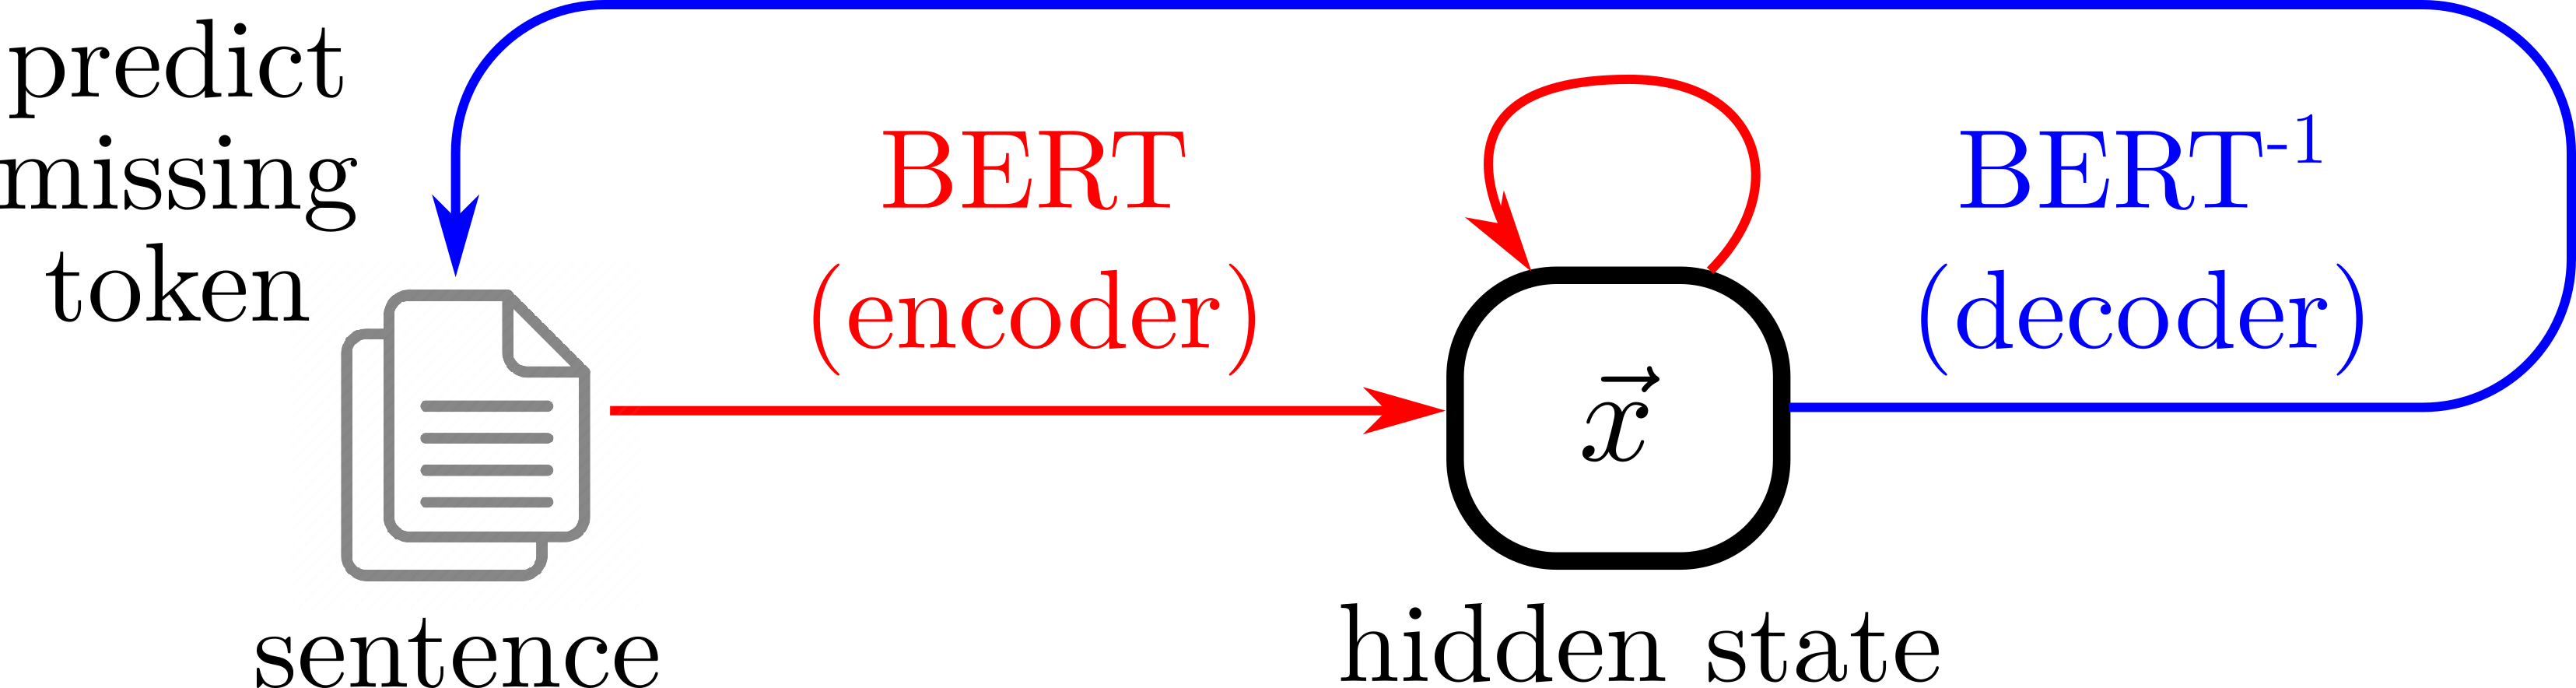
\includegraphics[scale=0.5]{BERT-architecture.png}}}
	\end{equation}
	换句话说: 隐状态的 representation 压缩了句子的意思,而它可以应用在别的场景下
	
	\item This implies that human-level AI can be \textit{induced} from existing corpora, 而\emp{不需重复 像人类婴儿成长的学习阶段}
	
	\item Such corpora can include items such as images, movies with dialogues / subtitles
	
	\item 这种训练方法是较早的另一篇论文提出,它并不属於 BERT 的内部结构
\end{itemize}
\end{frame}

\begin{frame}
\frametitle{从 BERT 过渡到 AGI}
\begin{itemize}
	\item \emp{词语} 组成 \emp{句子},类比於 逻辑中,\emp{概念} 组成 \emp{逻辑命题}
	
	\item 抽象地说,逻辑语言 可以看成是一种有 2个运算的 \emp{代数结构},可以看成是 加法 $\wedge$ 和 乘法 $\cdot$,其中 乘法 是不可交换的,但加法 可交换

	\item 例如 两个命题:
	\begin{equation}
	\mbox{我} \cdot \mbox{爱} \cdot \mbox{妳} \; \wedge \; \mbox{妳} \cdot \mbox{爱} \cdot \mbox{我}
	\end{equation}

	\definecolor{darkgreen}{rgb}{0.1, 0.5, 0.2}
	\item 这种逻辑结构 可以用 \emp{两层} 的 BERT 模型 处理:
	\begin{equation}
	\vcenter{\hbox{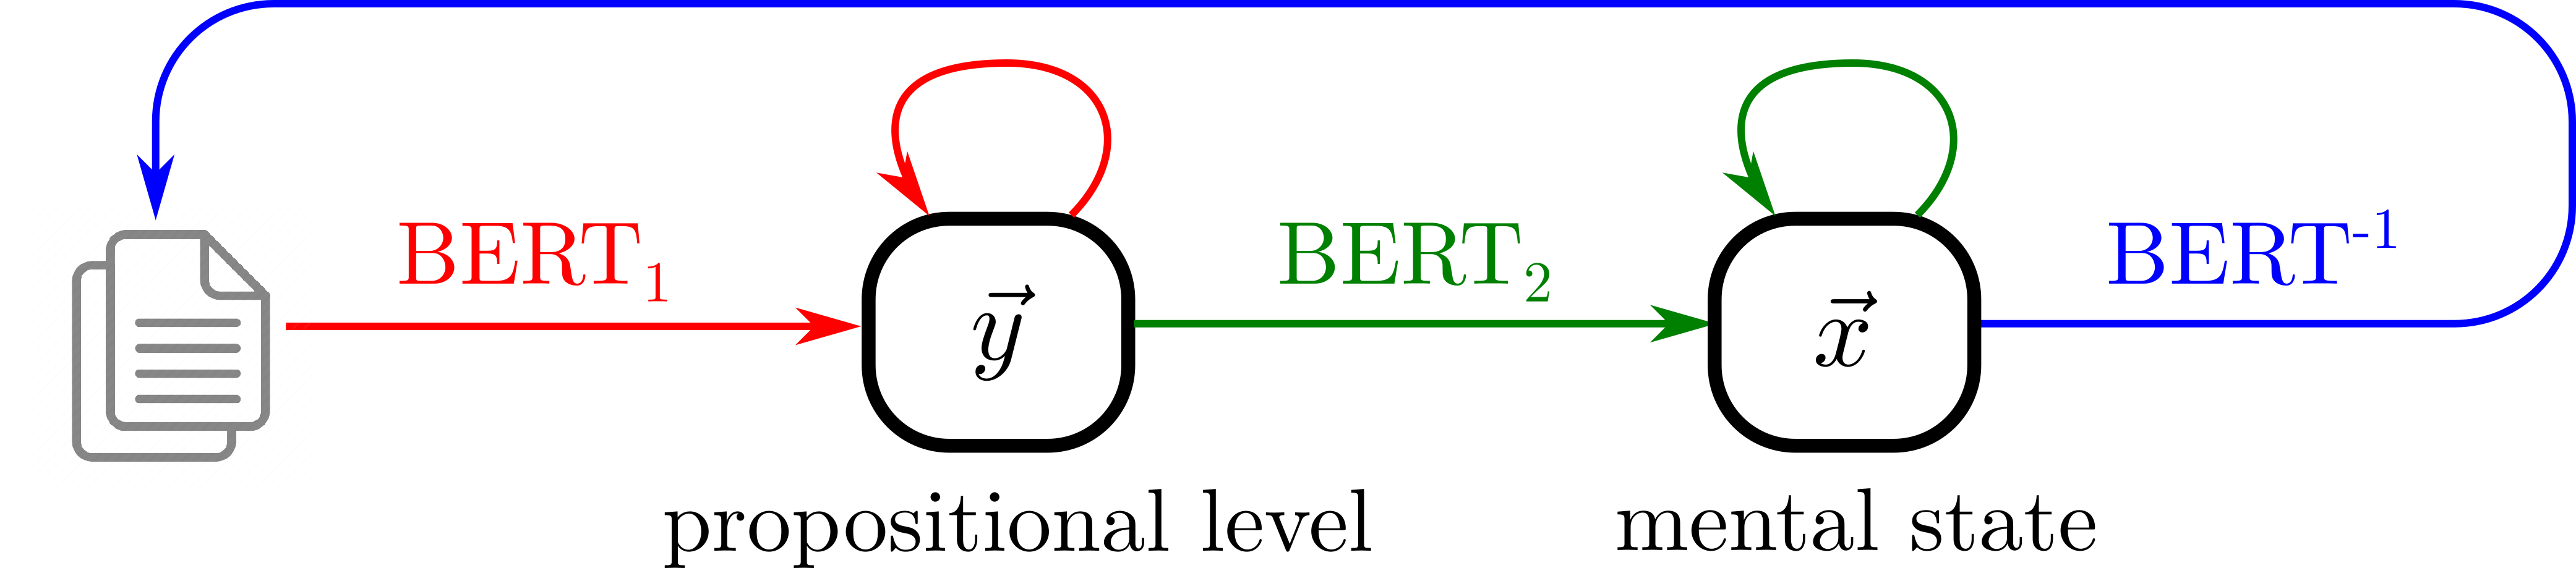
\includegraphics[scale=0.5]{2-BERT-architecture.png}}}
	\end{equation}
	({\color{red}第一层}似乎可以纳入到{\color{darkgreen}第二层},简化整个模型)

	\item 我发现 最难处理的问题,是在第2层 的状态 $\vec{x}$.  它是一个 逻辑命题 的 \emp{集合},集合中元素有可交换性,亦即 \emp{permutation invariance}.  这看似简单的特性,其实带来很大的麻烦

	% \item 如何 standardize 输入空间,使之可以接受任何形式的输入?
	
	% \item BERT 后端的输出可以是 actions,变成一个可以行动的 agent.  如何找大量的资料 训练它?

	% \item state $\vec{x}$ 的结构: 用 vector 还是 graph $\cong$ set of logic propositions 比较好? \\
	% 后者有 内在的 逻辑结构,是一种 inductive bias

	% \item 现时,所有 知识存在於 BERT 的 weights 里面,可不可以将一部分记忆 转化成 declarative knowledge,储存在 knowledge graph? 这做法有没有好处? 
\end{itemize}
\end{frame}

\begin{frame}
\frametitle{「集」结构 带来麻烦}
\begin{itemize}
	\item Word2Vec 也是革命性的; 由 Word2Vec 演变成 Sentence2Vec 则比较容易,基本上只是 向量的 \emp{延长} (concatenation); 逻辑命题 类似於 sentence

	\item 假设 全体逻辑命题的空间是 $\mathbb{P}$,则 \emp{命题集合} 的空间是 $2^{\mathbb{P}}$,非常庞大
	
	\item 如果限制 状态 $\vec{x}$ = working memory 只有 10 个命题,$\vec{x}$ 的空间是 $\mathbb{P}^{10}/\sim$ 其中 $\sim$ 是对称群 $\mathfrak{S}_{10}$ 的等价关系。 换句话说 $ 2^{\mathbb{P}} \cong \coprod_{n=0}^{\infty} \; \mathbb{P}^n / \mathfrak{S}_n $
	
	\item $\mathbb{P}^n / \mathfrak{S}_n$ 虽然是 $\mathbb{P}^n$ 的商空间,但 $\mathfrak{S}_n$-不变性 很难用神经网络实现

	\definecolor{darkgreen}{rgb}{0.1, 0.7, 0.2}
	\item 现时 比较可行的办法,是将 状态 $\vec{x}$ 实现成 一个时间上的「轮盘」,每个 ${\color{darkgreen}\bullet}$ 表示一个命题:
	\begin{equation}
	\vcenter{\hbox{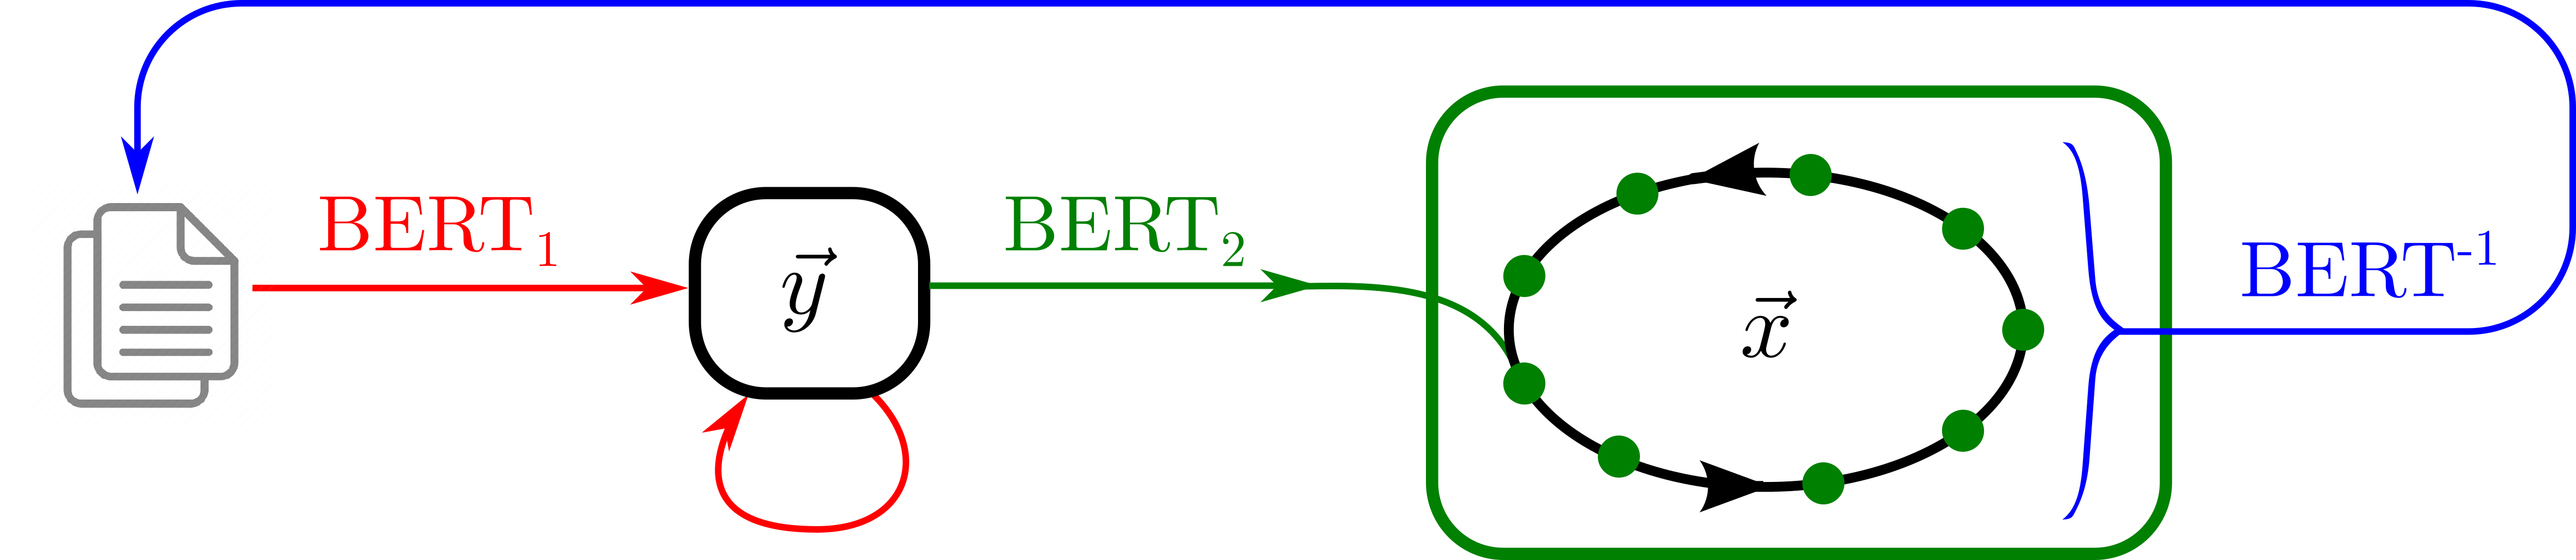
\includegraphics[scale=0.5]{BERT-with-carousel-architecture-1.png}}}
	\end{equation}

	\item 有趣的是,如果用「轮盘」方法,BERT 的 \emp{注意力机制} 有特殊意义....
\end{itemize}
\end{frame}

\begin{frame}
\frametitle{Attention 是什么?}
\begin{itemize}
	\item 注意力 最初起源於 Seq2seq,后来 BERT 引入 self-attention

	\item 在 Seq2seq 中,编码器 (encoder) 由下式给出,它将输入的词语 $x_i$ 转化成 一连串的 隐状态 $h_i$:
	\begin{equation}
	h_t = \mbox{RNN}_{encode}(x_t, h_{t-1})
	\end{equation}

	\item 这些 $h_i$ 可以综合成单一个 隐状态 $c = q(h_1, ..., h_n)$. 

	\item 这个 $c$ 被「寄予厚望」,它浓缩了整个句子的意义
	
	\item 解码器 的结构类似,它的隐状态是 $s_t$,输出 $y_t$:
	\begin{equation}
	s_t = \mbox{RNN}_{decode}(y_t, s_{t-1}, c_t)
	\end{equation}
	
	\item 注意最后的 $c_t$ 依赖时间,它是隐状态 $h_j$ 的 \emp{加权平均}:
	\begin{equation}
	c_i = \sum_j \alpha_{ij} h_j
	\end{equation}
	
	\item 其中 $\alpha_{ij}$ 量度 输入/输出 的隐状态之间的 \emp{相似度},取其最大值:
	\begin{equation}
	\alpha_{ij} = \mbox{softmax} \{ \langle s_i, h_j \rangle \}
	\end{equation}
	换句话说,$\alpha_{ij}$ \emp{选择} 最接近 $h_j$ 的 $s_i$
\end{itemize}
\end{frame}

\begin{frame}
\frametitle{Attention 给逻辑 AI 的启发}
我这样理解 attention:
\begin{itemize}
	\item 例如,翻译时,输入/输出句子中「动词」的位置可以是不同的
	
	\item 当 解码器需要一个「动词」时,它的隐状态 $s_t$ 含有「动词」的意思
	
	\item Attention 机制 找出最接近「动词」的 编码器的隐状态 (可以 $\ge 1$ 个)$\sum h_j$,交给 解码器,这是一种 \emp{information retrieval}
	
	\item 例如,将 $M$ 件东西 映射 到 $N$ 件东西,可以有 $N^M$ 个 mappings,这是非常庞大的空间。 但如果这些物件有 \emp{类别},而\underline{同类只映射到同类},则可以用 attention 简化 mappings
	
	\item 所以 attention 是一种 inductive bias,它大大地缩小 mapping 空间

	\item 在逻辑的场景下,需要的 mapping 是 $f: \mbox{命题集合} \rightarrow \mbox{命题}$
	\begin{equation}
	\vcenter{\hbox{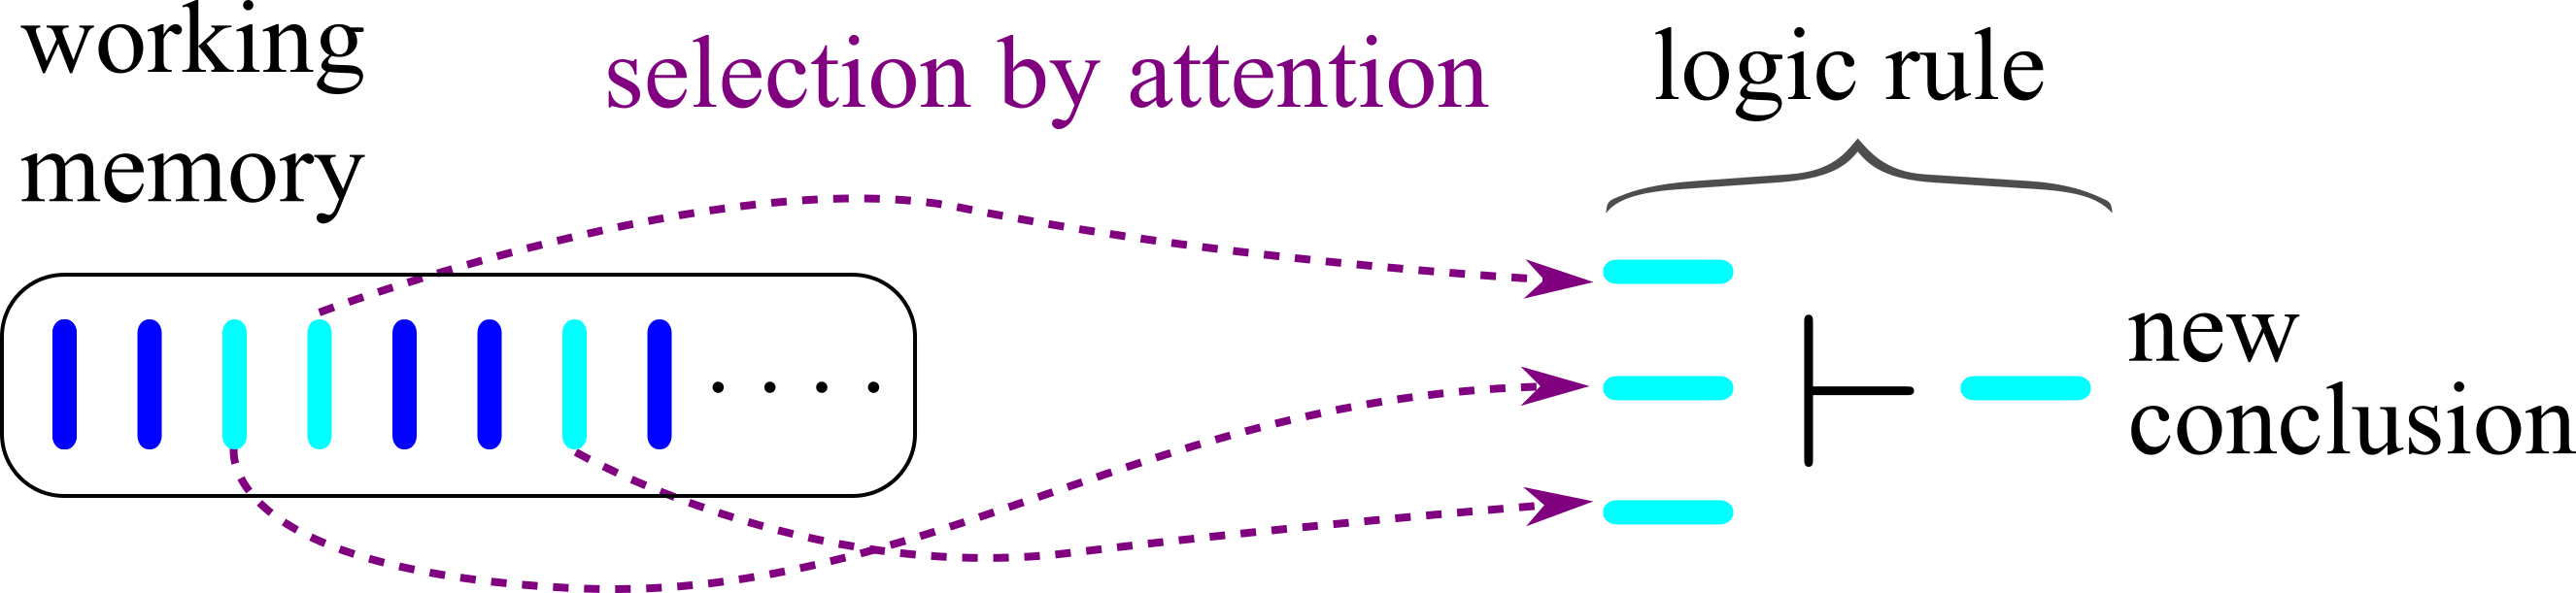
\includegraphics[scale=0.5]{attention-in-logic.png}}}
	\end{equation}

\end{itemize}
\end{frame}

\begin{frame}[plain]
\frametitle{Attention... is not what we want}
\begin{itemize}
	\item 逻辑 attention 和 传统 attention 要求略有不同,这是关键的一步

	\item 不是「同类映射到同类」,而是要在庞大的 logic rules 空间中找到适用(applicable)的 rules

	\item 隐状态 $s_t$ 代表 ``search state'',注意力 的目的是 \emp{选择} $s_t$ 所需要的那些命题,交给 解码器

	\item 注意: 逻辑 attention 从 $M$ 个命题中 选择 $N$ 个命题,$M > N$. 这是 inductive bias. \ 而 Symmetric NN 的做法,只是要求 $M$ 个命题 的 \emp{置换不变性},所以它浪费了资源在很多 ``don't care'' 的命题上

	\item 换句话说,selection 所带来的 bias 如果足够强,似乎不需要 symmetric. \  很巧合地,再次应验了 ``attention is all you need'' 这句话
\end{itemize}
\end{frame}

\begin{frame}
\frametitle{Fourier 神经网络}
\begin{itemize}
	\item 之前说过,需要 symmetric 神经网络。 可以用 \emp{多项式} 激活函数,得出一大堆 多项式的 weight-sharing 条件。 这方法在 层数 增大时,计算变得很复杂。 这是一个 computational invariant theory 的问题,我暂时未有时间深入研究
	
	\item 另一个方法我称之为 Fourier 神经网络
	\item 命题空间 $\mathbb{P}\mathrm{rop}$
\end{itemize}
\end{frame}

\begin{frame}
\frametitle{「神经」知识表示}
为什么要研究 神经知识表示?
\begin{itemize}
	\item 从经典 logic-based AI 的传统,一直在使用「符号」的知识表示法

	\item 符号逻辑 很容易转换成 抽象代数/范畴论 形式(它们是同一个大家庭的「近亲」)
	
	\item 然而 或许存在 截然不同 的知识表示法? 但我们很难想像它 \emp{长什么样子}

	\item 人脑的「神经」知识表示,可以作为参考,然后再研究它和逻辑表示之间的 correspondence
\end{itemize}

\vspace*{0.4cm} 神经知识表示 的特点:
\begin{itemize}
	\item distributive(分布性)

	\item model-based (vs rule-based)

	\item \textit{in situ}(固定性)--- 例如辨认「猫」的时候,大脑中 相应的神经元被 激活,但这些 神经元 \emp{不能移动},所以「猫」的表示 也不可移动
\end{itemize}
问题是: 如果要辨认「白猫追黑猫」,「猫」的表示是固定的,则这两个「猫」表示 如何\emp{共存}於神经网络中?\\
答案很可能是: 两个「猫」\emp{交替}地 出现在 \emp{时间}上
\end{frame}

\begin{frame}
\frametitle{神经 特征簇 (feature clusters)}
例如,以「匙羹在杯中」作例子:
\begin{equation}
	\vcenter{\hbox{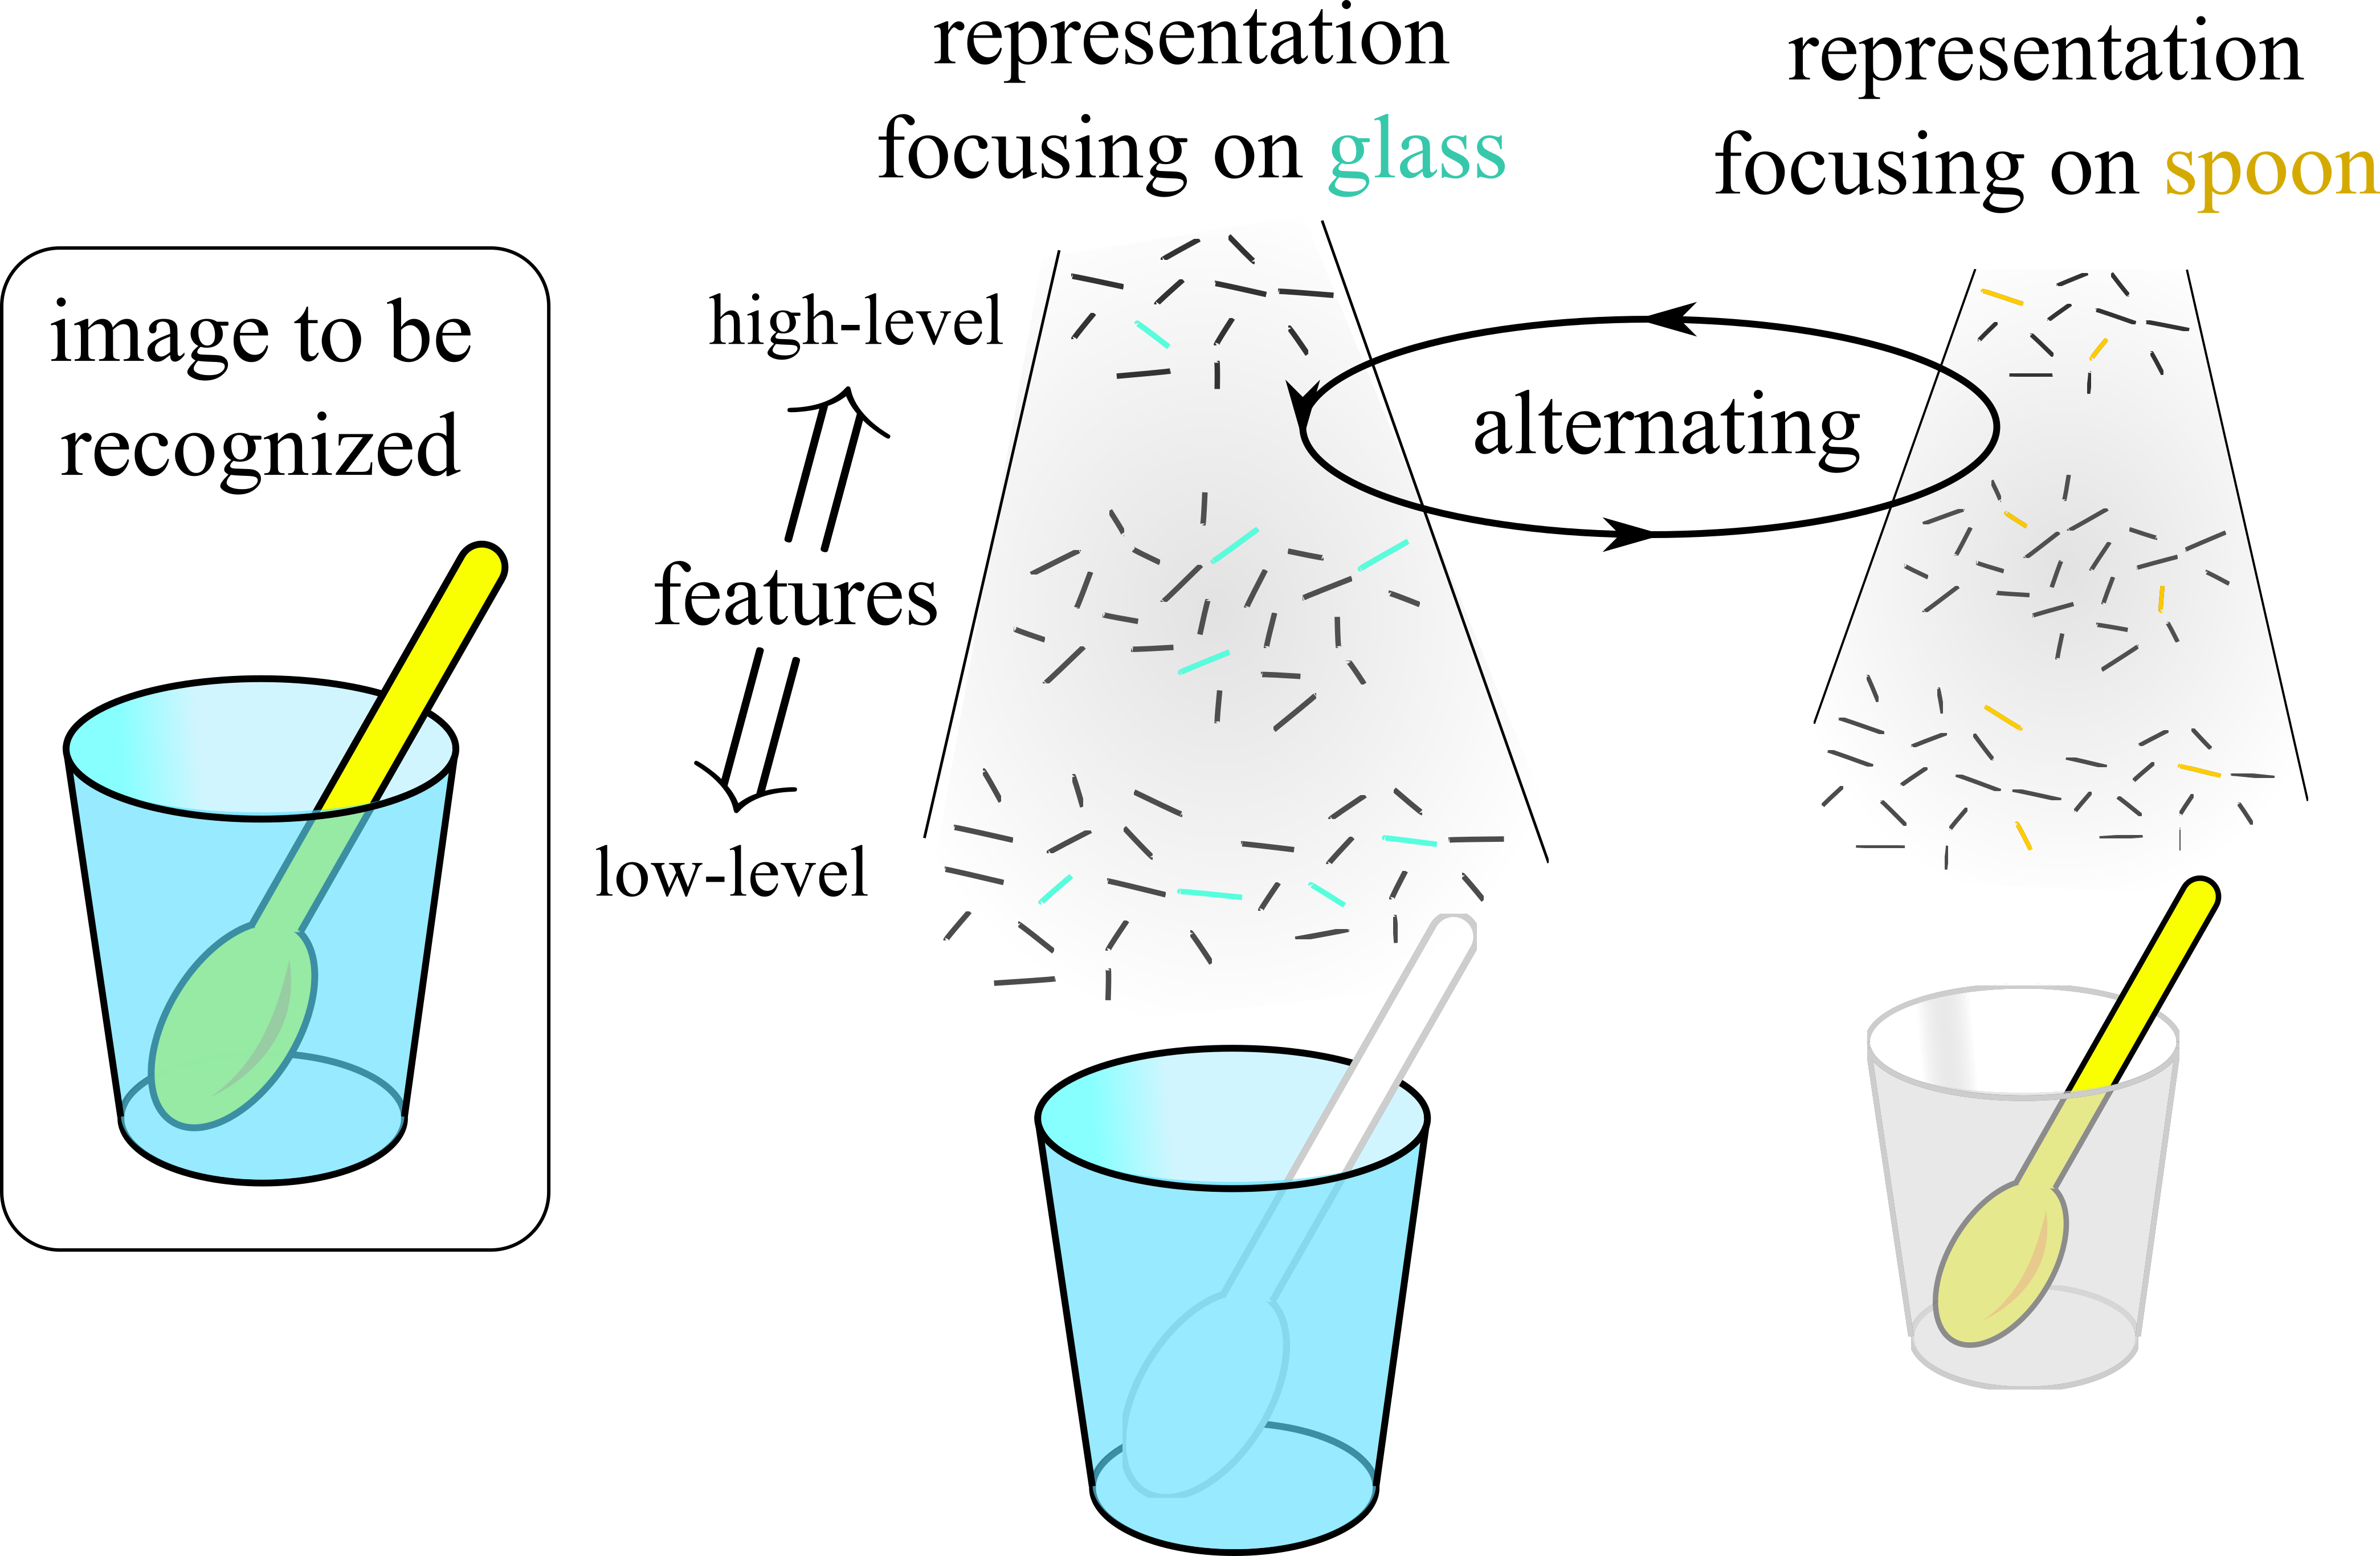
\includegraphics[scale=0.5]{neural-representation-alternating-glass-spoon.png}}}
\end{equation}
每个 复杂物体 由一个 \emp{feature cluster} 辨认。 多个「特征簇」在时间上交替出现,可以看成是一种 composition,例如 $A \cdot B$ 或 $A \circ B$.
\end{frame}

\begin{frame}
\frametitle{高阶 特徵}
\begin{itemize}
	\item 一串 特征簇 的时间序列,例如 $A \cdot B$,可以被 更\emp{高阶} 的神经网络 用作输入。 高阶辨认 的结果是一些关系 (relations),例如「匙羹\emp{在}杯\emp{内}」
	\begin{equation}
		\vcenter{\hbox{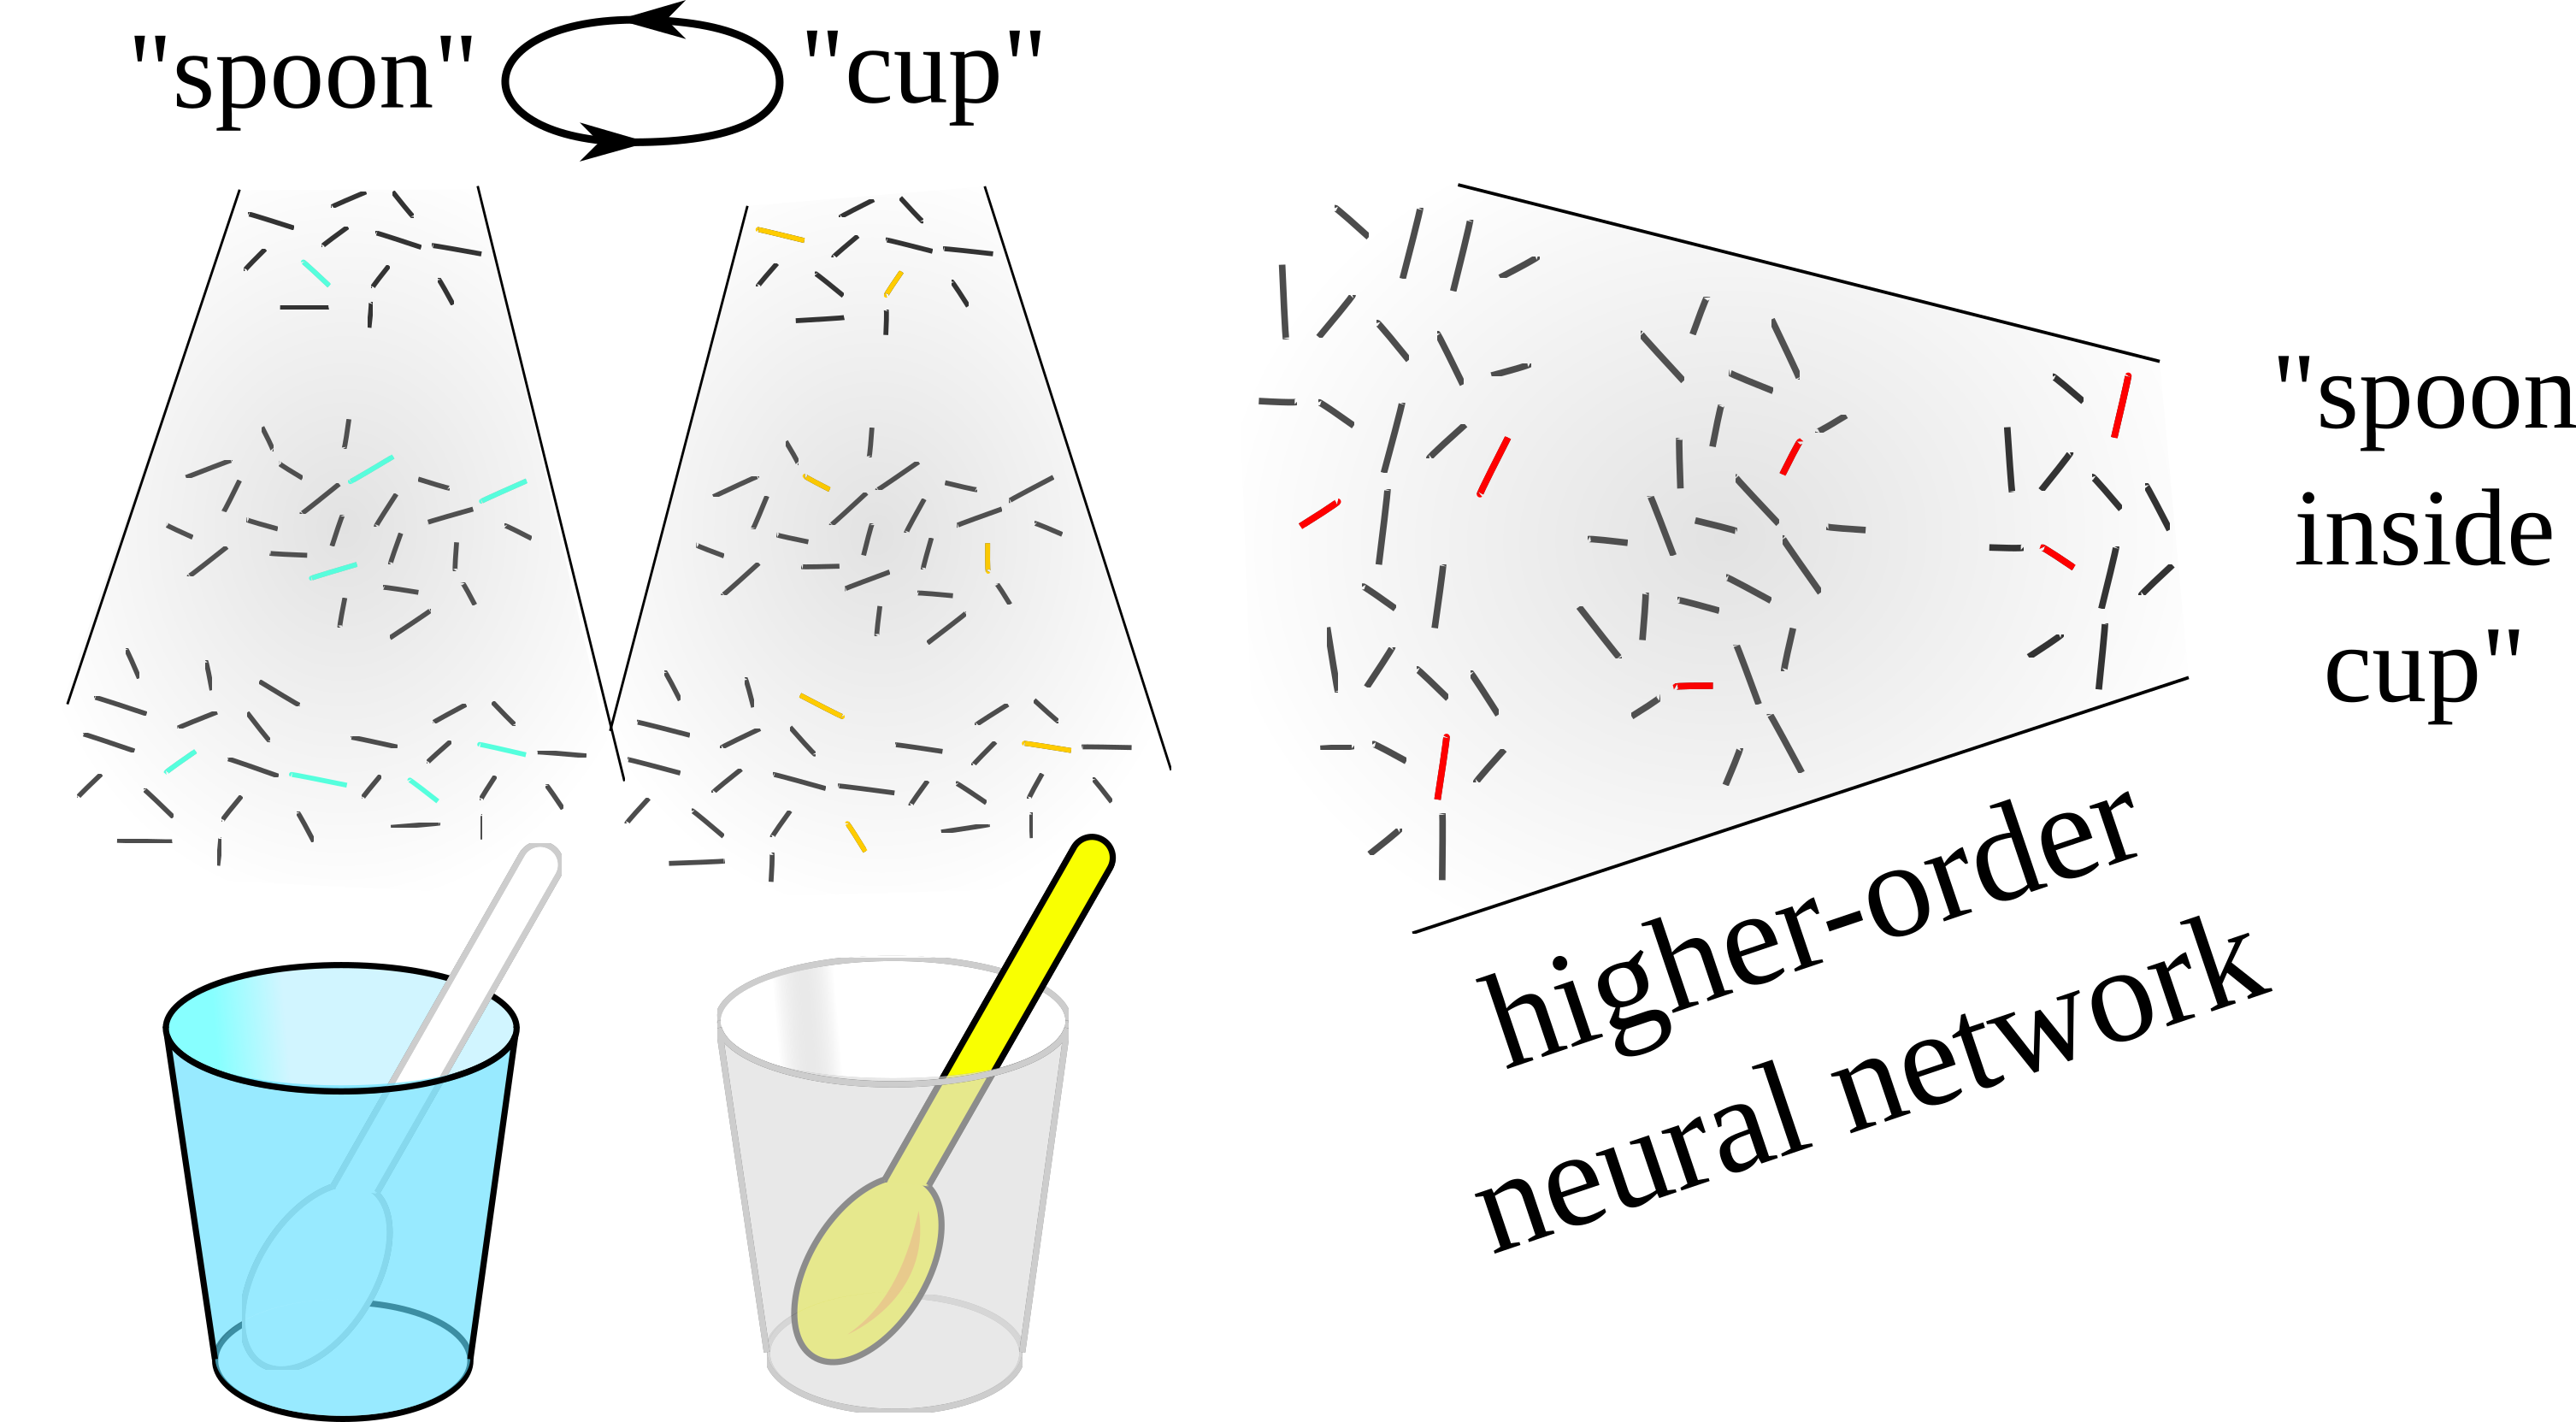
\includegraphics[scale=0.5]{higher-order-NN.png}}}
	\end{equation}
	
	\item 这似乎是一个 $\mbox{特征空间} \times \mbox{时间}$ 的映射 $f: X \times T \rightarrow Y$
	
	\item {\color{red}关於这部分其实我仍未肯定,或许有其他方法}
\end{itemize}
\end{frame}

\begin{frame}
\frametitle{神经 $\leftrightarrow$ 逻辑 correspondence}
\begin{itemize}
	\item 我们的目标是了解 神经表示 和 逻辑表示 之间的关系,这关系或许可以用范畴论描述?
	
	\item 定义 复杂情境 (complex scenario) 是 感知材料 (sensory data) 的一个片段,如:
	\begin{equation}
		\vcenter{\hbox{
\includegraphics[scale=0.5]{sensory-movie.png}}}
	\end{equation}
	又或者一个故事,例如「John 爱 Mary 但 Mary 不爱他」
	
	\item 一个复杂情境 可以用若干个 特征簇 描述
	
	\item Equivalently, 复杂情境 可以用 \emp{逻辑} 表示,就是一大堆 逻辑命题 的 conjunction,这些命题 钜细无遗 地描述该情境
\end{itemize}
\end{frame}

\begin{frame}
\frametitle{再谈一次 逻辑结构}
\begin{itemize}
	\item 以前曾经说过,机器视觉 的成功,有赖於 将 视觉的几何结构 impose 在深度神经网络上
	\item 这 深度神经网络 原本是 ``free'' 的,但加了限制之后,权重空间 变小了(例如维数降低),所以学习加速了
	\item 所谓 symmetry 的意义,简单例子:「如果知道左边等於右边,那就只需计算一次」
	\item 换句话说,数学家喜欢对称性,是因为它经常可以简化计算
	\item 同理,我们想将 逻辑结构 的对称性 impose 到神经网络
	\item 实际上,可能只需要逻辑上的交换律,就可以达到 强人工智能,正如 机器视觉的成功,在於引入了 CNN 的 convolution 结构,后者只是 视觉不变性 的其中一个最显著的 invariant
	\item 现代逻辑理论 非常漂亮,我花了十多年时间才弄懂,我希望将这套 逻辑-学习 理论简单讲解一下,也算功德完满了
\end{itemize}
\end{frame}

\begin{frame}[plain]
\begin{itemize}
	\item 在经典时代,逻辑的 代数形式 可以用 Boolean algebra 表述,然而这方法只适用於 命题逻辑
	\item Boolean algebra 是中学生熟悉的,类似 Venn diagram 的结构
	\item 这种结构和 拓樸学 的 open sets 结构一样,所以 命题逻辑 也可以看成是一种 topology
	\item 然而 predicate logic 的结构更复杂,直到最近才有比较完善的表述
	\item 现代逻辑结构和 type theory 有深刻的关系,此即 Curry-Howard isomorphism
	\item 现代逻辑也涉及 topos theory,那是一种由 algebraic geometry 引入的结构
\end{itemize}
\end{frame}

\begin{frame}
\frametitle{Type theory and the Curry-Howard isomorphism}
\begin{itemize}
	\item 大家都知道 Lisp 语言没有 type,它是一种 untyped $\lambda$-calculus
	\item 在 Lisp 之上引入 type system,衍生成 ML, Caml, OCaml, Haskell 等 一系列语言
	\item 每一个 program 属於某个 type,例如 $\mathrm{length}()$ 函数,输入一个字串,输出它的长度; $\mathrm{length} : \mathsf{String} \rightarrow \mathsf{Integer}$
	\item 有些逻辑学家 察觉到 类型论 的 $\tau_1 \rightarrow \tau_2$ 和逻辑中 $P \rightarrow Q$ 是一模一样的
	\item 这个关系的发现者至少包括 Brouwer-Heyting-Kolmogorov-Curry-Howard
	\item 这关系的深刻之处,在於把 符号逻辑上的 proofs 和 程式语言 的 programs 划上等号,前者是 符号/静态的,后者是 程序/动态的
	\item 每个 proof 就是一个 program,它输入一些 arguments,输出 关於那些 arguments 的证明
	\item 例如: 「所有人都会死」是一个 program,它输入「苏格拉底」,输出「苏格拉底会死」 
	\item 这个对应正好可以应用到深度学习: 神经网络 是一个 function mapping,它将 逻辑前提 map 到结论
\end{itemize}
\end{frame}

\begin{frame}
\frametitle{Topos theory and fibrations}
\begin{itemize}
	\item Predicate logic (谓词逻辑)和 命题逻辑 之间的差异在於 fibration 结构
	\item Fibration 通常用 $\mathrel{\substack{\mathbb{E}\\\downarrow \\\mathbb{B}}  {\scriptstyle \pi}}$ 表示,$\mathbb{B}$ = base space, $\mathbb{E}$ = \'{e}tale space, $\pi$ = projection
	\item Base space 是 type 的空间,\'{e}tale space 是 predicate 的空间
	\item 例如 $\mathbb{B}$ 空间的一个 type 是 $\mathrm{Human}$,$\mathbb{E}$ 空间的一个谓词是 $\mathrm{Mortal}$
	\item 於是有以下这个 type inference rule:
	\begin{equation}
	i:\mathrm{Human} \vdash \mathrm{Mortal}(i): \mathsf{Prop}
	\end{equation}
	意思是说,如果 $i$ 属於 $\mathrm{Human}$ 类型,则 $\mathrm{Mortal}(i)$ 属於 $\mathsf{Prop}$ 类型
	\item Topos 是一种 Cartesian-closed category (CCC)
	\item 
\end{itemize}
\end{frame}

\frame[allowframebreaks]{
\cc{多谢收看}{Thanks for watching} \smiley
% \frametitle{References}
\printbibliography
}

\end{document} 